\input{doctools/latex/magazine_template.tex}   %Page setup
\input{doctools/latex/mycommands.tex}       %Some useful commands

% Figure search path
\graphicspath{
              {figs/} % Figures drawn with xfig
              {pngs/} % Other graphics files
}

% Use \draftnote to mark the filenames of figures
\newcommand{\isdraft}{1} %Choose 1 for draft, 0 for release
\doublespacing{} % Double space the document for proofreading
\begin{document}





%%%%%%%%%%%%%%%%%%%%%%%%%%%%%%%%%%%%%%%%%%%%%%%%%%%%%%%%%%%%%%%%%%%%
%Title
%%%%%%%%%%%%%%%%%%%%%%%%%%%%%%%%%%%%%%%%%%%%%%%%%%%%%%%%%%%%%%%%%%%%
\begin{center}
	{\huge ASCII command interface for the AVR Butterfly}\\
	\today
\end{center}



\section{Introduction}
I love test equipment with open, well documented, ASCII command sets.  The plain text commands give a complicated instrument a familiar interface and an easy way to automate measurements.  Python's gnuplot and pySerial interfaces let you acquire and make pretty plots of your data -- all for free\cite{pyserial,gnuplot-py}. So when I need to automate hobby measurements at home, I immediately wish for an ASCII interface to whatever tool I'm measuring with.  This tool happens to be the AVR Butterfly board right now, simply because it's cheap and the LCD is handy.  

\clearpage
\section{Working with the Butterfly}
The AVR Butterfly board consists of an AVR ATmega169 microcontroller and some peripherals.  Figure \ref{fig:connections} shows the connections I make to it.  I only use 3 wires from the DB9 connector for serial communication with the PC -- there's no hardware handshaking.  And while I could also use this serial channel for programming, I find that using a dedicated programmer makes iterating my code much faster.  A 6-pin header soldered to the J403 position lets me use Atmel's AVRISP mkII programmer.  Finally, powering the board with an external supply at J401 means that I don't have to think about the Butterfly's button cell battery.

After the hardware is connected, I use \textbf{avrdude}\cite{avrdude} and \textbf{GNU make}\cite{gnumake} to automate building the code and programming the Butterfly's flash memory.  I modified a makefile template from the WinAVR project\cite{winavr} to specify my part, programmer, and source files.  The comments in this template file were a big help for understanding how to customize it, and for understanding the build process in general.  Finally, I installed \textbf{avr-gcc} and other cross-compilation tools using Gentoo Linux's \textbf{crossdev} package.  I could have put these last pieces on ``by hand'', but \textbf{crossdev} convieniently updates the toolchain as new versions are released.     

\begin{figure}[ht]
    \begin{center}
        \includegraphics[clip,scale=1]{usart_pinout}
        \draftnote{usart\_pinout.fig}
        \caption{Connections needed for the AVR Butterfly.  The AVRISP mkII user's guid stresses that the programmer must be connected to the PC before the target (Butterfly board).  The code presented here configures the USART for 9600 baud, 8 data bits, 1 stop bit, no parity checks, and no flow control. \label{fig:connections}}
    \end{center}
\end{figure}

\clearpage
\section{Handling incoming characters}
Receiving remote commands begins with receiving characters, which are sent to the AVR via the USART connector shown in figure \ref{fig:connections}.  Reception of these characters triggers an interrupt service routine (ISR), which handles them according to the flow shown in figure \ref{fig:recflow}. The first step in this flow is loading the characters into the receive buffer.

Figure \ref{fig:recbuffer} illustrates the receive buffer loaded with a combined string.  The buffer is accessed with a pointer to its beginning and a second pointing to the next index to be written.  These pointers are members of the \texttt{recv\_cmd\_state\_t} type variable \texttt{recv\_cmd\_state}.  This is just style -- I like to try to organize varibles used in a flow by making them members of their own structure.  Naming conventions aside, it's important to notice that there's no limitations on command or argument size imposed in this first step, provided that the total character count stays under the \texttt{RECEIVE\_BUFFER\_SIZE} limit. 
 
When a combined string in the receive buffer is finished with a carriage return, the string is copied over to a second buffer.  I call this the parse buffer, since this is where the string will be searched for recognized commands and arguments.  This buffer is locked until its contents can be processed to keep it from being clobbered by new combined strings.  Sending commands faster than they can be processed will generate an error, and combined strings sent to a locked parse buffer will be dropped.  The maximum command processing frequency will depend on the system clock and other system tasks.  

\begin{figure}[ht]
    \begin{center}
        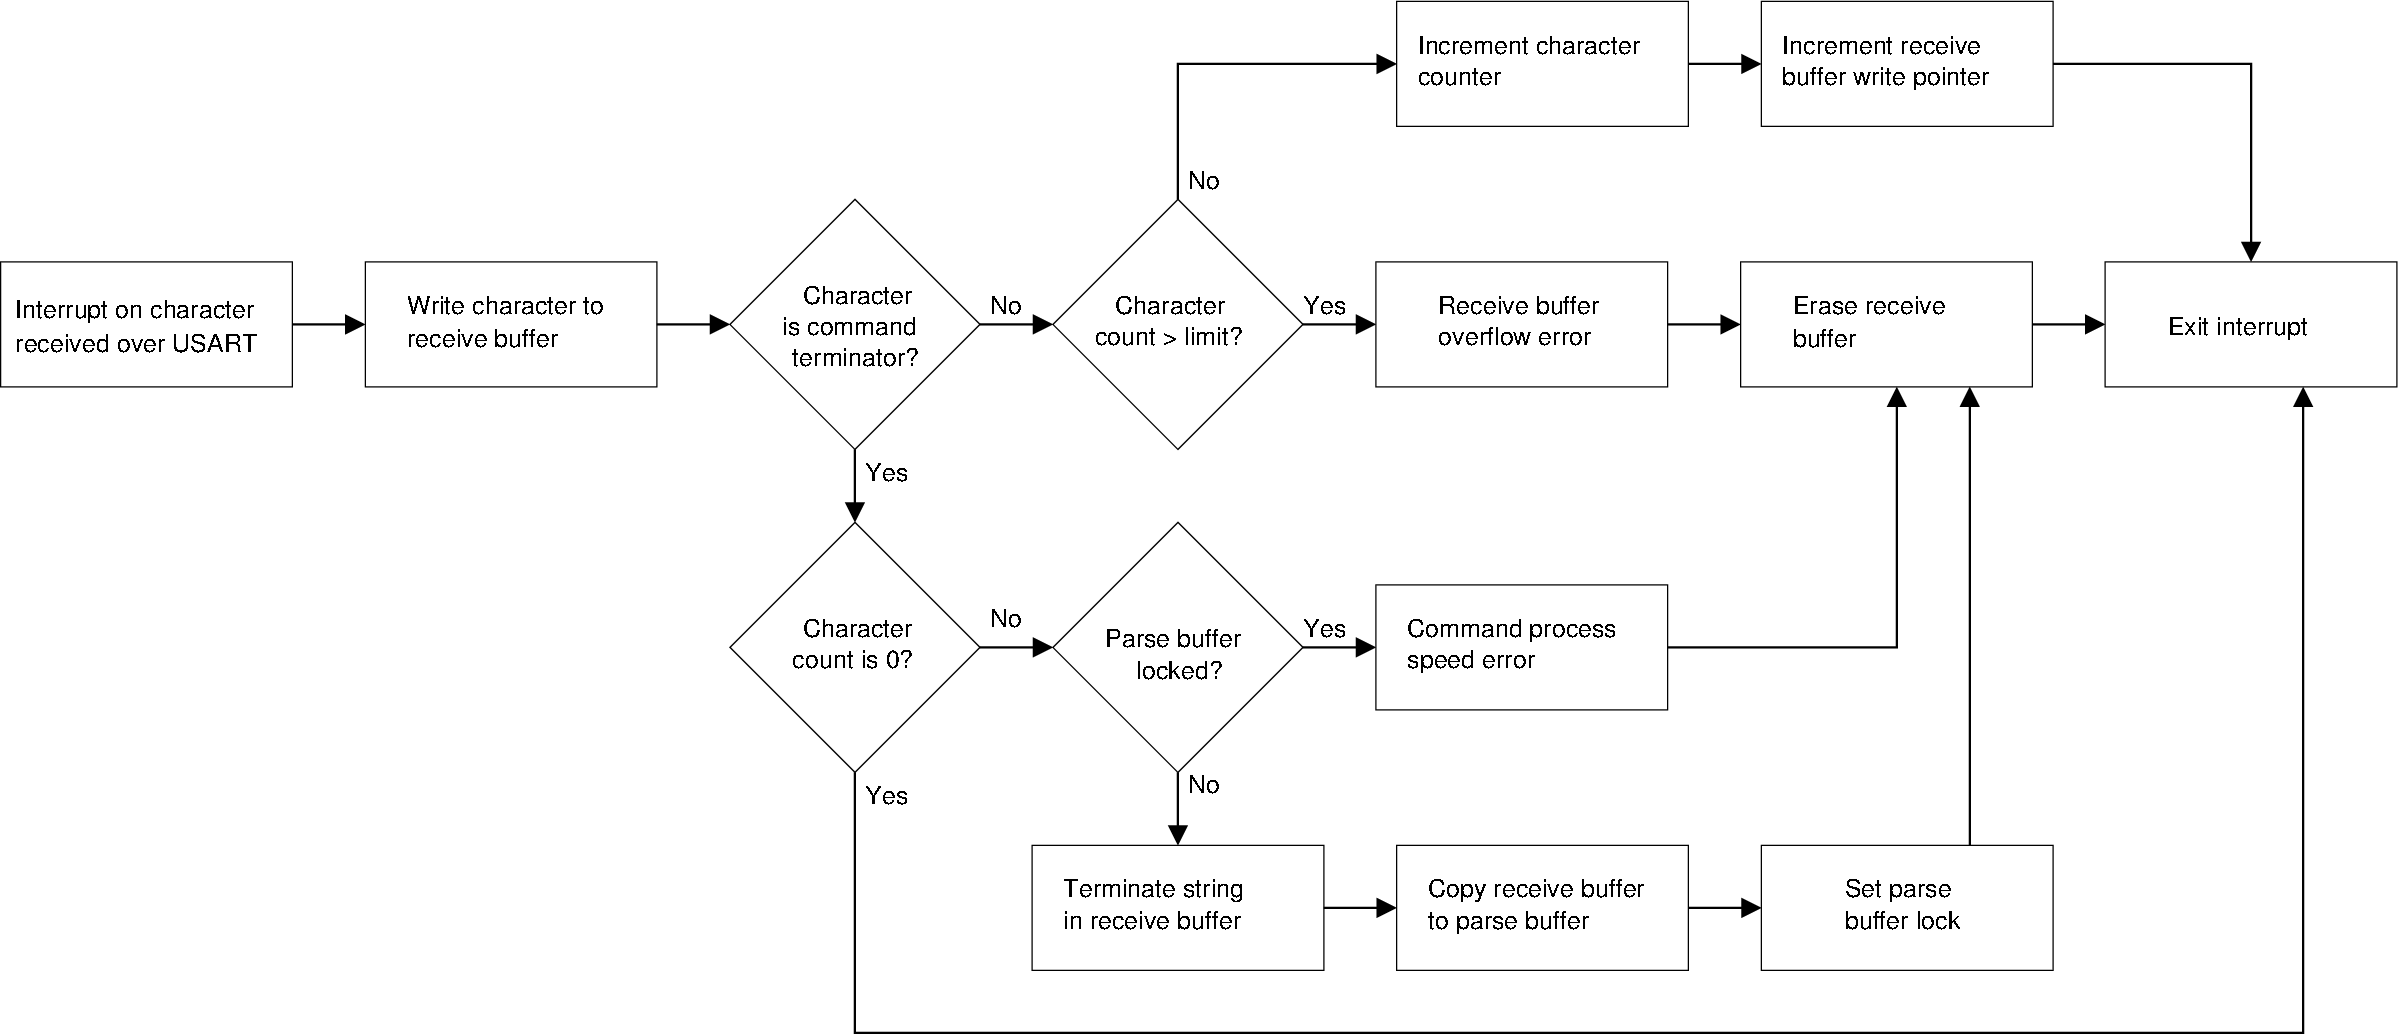
\includegraphics[clip,scale=0.8]{./tikz/recv_cmd_flow}
        \draftnote{recv\_cmd\_flow.tex}
        \caption{Program flow for processing characters received over the Butterfly's USART.  Sending a command terminator (carriage return) will always result in an empty receive buffer.  This is a good way to make sure there's no garbage in the buffer before writing to it.\label{fig:recflow}}
    \end{center}
\end{figure}

\begin{figure}[ht]
    \begin{center}
        \includegraphics[clip,scale=1.1]{recbuffer}
        \draftnote{recbuffer.fig}
        \caption{The received character buffer and pointers used to fill it.  There is no limit to the size of commands and their arguments, as long as the entire combined string and terminator fit inside \texttt{RECEIVE\_BUFFER\_SIZE}.\label{fig:recbuffer}}
    \end{center}
\end{figure}

\clearpage{}
\section{Watching the progress}
I set up a logging system to help me understand how commands were being processed.  It's inconvenient to have the command and logging interfaces share the same communication channel, but the Butterfly only has one USART.  Reading command replies back without getting confused by general log messages requires some control over how the logging system works.  For now, figure \ref{fig:hellotrace} shows the system processing the ``hello'' command with logging enabled at its most verbose level.  Each log message is tagged with a character representing the message severity (information, warning, error), followed by a string representing the subsystem responsible for the message.  These tags can be used to adjust what log messages should be suppressed, though I won't go into that here.  The ``Hello yourself!'' reply isn't a log message, and thus has no tags.

I should mention that these log message strings can easily overwhelm the Butterfly's RAM if they're not stored and referenced in flash memory.  Savannah\cite{url:savannah:pgmspace} and Dean Camera\cite{url:deancamera:pgmspace} have written great instructions for using the pgmspace module to handle this problem.  This module supplies the PROGMEM and PSTR macros I use throughout my code.

% Send characters to the butterfly using the hellotrace.py script in the
% pngs directory.  Then use the termgrab.sh script to create hellotrace.eps.
\begin{figure}[ht]
    \begin{center}
        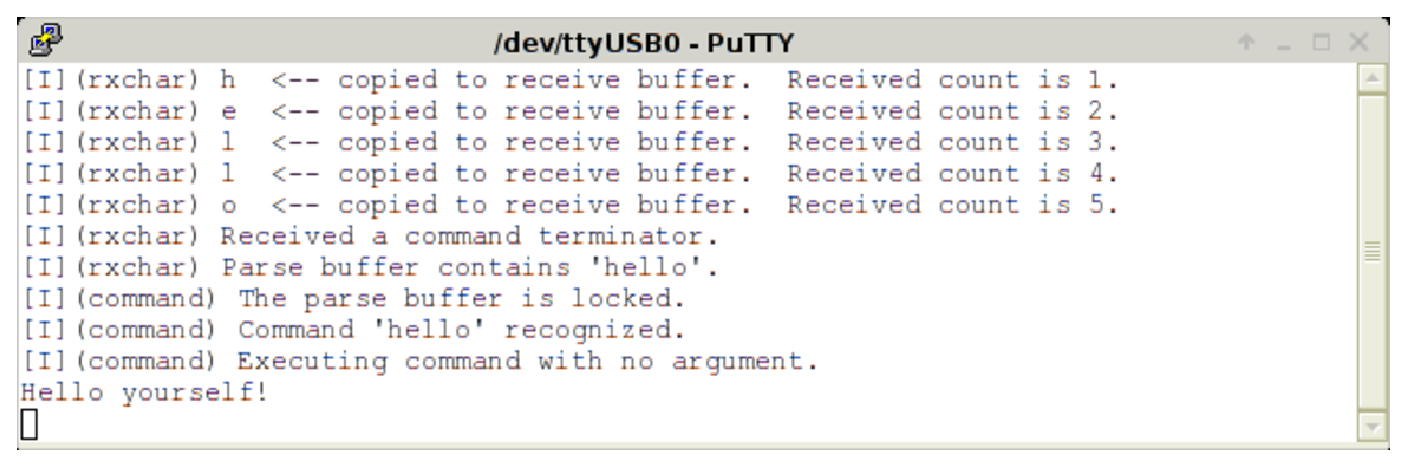
\includegraphics[clip,scale=0.5]{pngs/hellotrace.eps}
        \draftnote{hellotrace.eps}
        \caption{Terminal output showing the reception of and the reply to the ``hello'' command.  The logging system has been set to its most verbose level, so you see ``unsolicited'' messages as well as the command reply.  These messages can be suppressed by clearing bits in the logger configuration register.\label{fig:hellotrace}}
    \end{center}
\end{figure}

% Using the logger section.  Should describe the log levels and the log systems.
\clearpage{}
\section{Configuring the logger}
The logger acts as a gatekeeper for messages emitted from other subsystems.  In the output shown in figure \ref{fig:hellotrace}, the \texttt{command} subsystem has a lot to say about every character received over the USART.  At 9600 buad, sending an 80-character message (10 bits per character) takes almost 100 milliseconds.  The processor will not be able to handle new commands during this time, as it won't get around to processing the parse buffer.  So we need to suppress messages we don't need to see.  

Messages are sent to the logger using the \texttt{logger\_msg\_p} function, where the \texttt{\_p} suffix indicates that the message must be stored and referenced in flash memory.  These messages are tagged with the origin subsystem and a severity level.  These two tags have corresponding members in the logger configuration structure, which the logger consults while deciding whether or not to print the message.  I should have remote commands to let the user set each of these members, but I only have a command to enable the subsystem right now.  I wanted to keep the command array short for this article.  For now, I just have a function defined to set the severity configuration.   

The logger first checks to see if the incoming message's severity is at or above the configuration level.  This level is an enumerated type, with the \texttt{log\_level\_INFO} member given the lowest value and \texttt{log\_level\_ERROR} given the highest.  If the severity is high enough, the logger checks to see if the message's subsystem has been enabled for logging.  Subsystem tags are recognized by comparing the tag string with strings in the logger module's system array.  Each subsystem has one bit in a 16-bit register.  Setting the bit enables the subsystem's messages, and clearing it suppresses them.  The \texttt{logreg} remote command allows users to set bits in this register while the system is running.  Of course, the system's documentation has to match up bit positions with subsystems for this command to be useful. 

Each subsystem needs an entry in the logger's subsystem array for this scheme to work.  It might be nice to automate the creation of this array so that the programmer doesn't have to think about it when adding a new subsystem.  For now, the logger module must be made aware of new subsystems by manually adding these array entries.
      

\clearpage{}
\section{Recognizing commands}
After finished combined strings are copied from the receive to the parse buffer, the system separates them into command and argument strings using the flow shown in figure \ref{fig:cmdflow}.  Commands in the parse buffer are then separated from their arguments with a string terminator inserted into the first space between the two.  As illustrated in figure \ref{fig:prsbuffer}, pointers to the beginning of the parse buffer and the beginning of the argument will then reference two separate strings.  The first of these two, the command string, is converted to lowercase and compared with those in the command definition array to look for a match.

The lower section of listing \ref{lst:cmdsnip} shows my simple command definition array with entries for the ``hello,'' ``logreg,'' and ``help'' commands. The structure of this array is largely taken from White\cite{bok:white2012}.  Each entry must be of the type \texttt{command\_t}, defined in the upper section of listing \ref{lst:cmdsnip}.  Notice that the function pointer member of this command type only accepts one integer argument.  This can be changed to make the system more flexible, but remember that every function called by remote commands must accept the same arguments.  If the function pointer is expanded to accept both an integer and a string pointer argument, all of the functions the pointer will point to must also be expanded.  

The other members of the command type contain the command's name (must be lowercase), its argument type, the maximum number of characters in the argument, and a help string.  The argument type tells the command processing system how it should handle the argument string.  Hexadecimal argument strings, for example, are converted to integers before being passed on.  The character limit is a basic way of limiting incoming arguments.  Finally, the help string is what is printed to the USART when the ``help'' command is issued.


% The parse buffer processing flowchart
\begin{figure}[ht]
    \begin{center}
        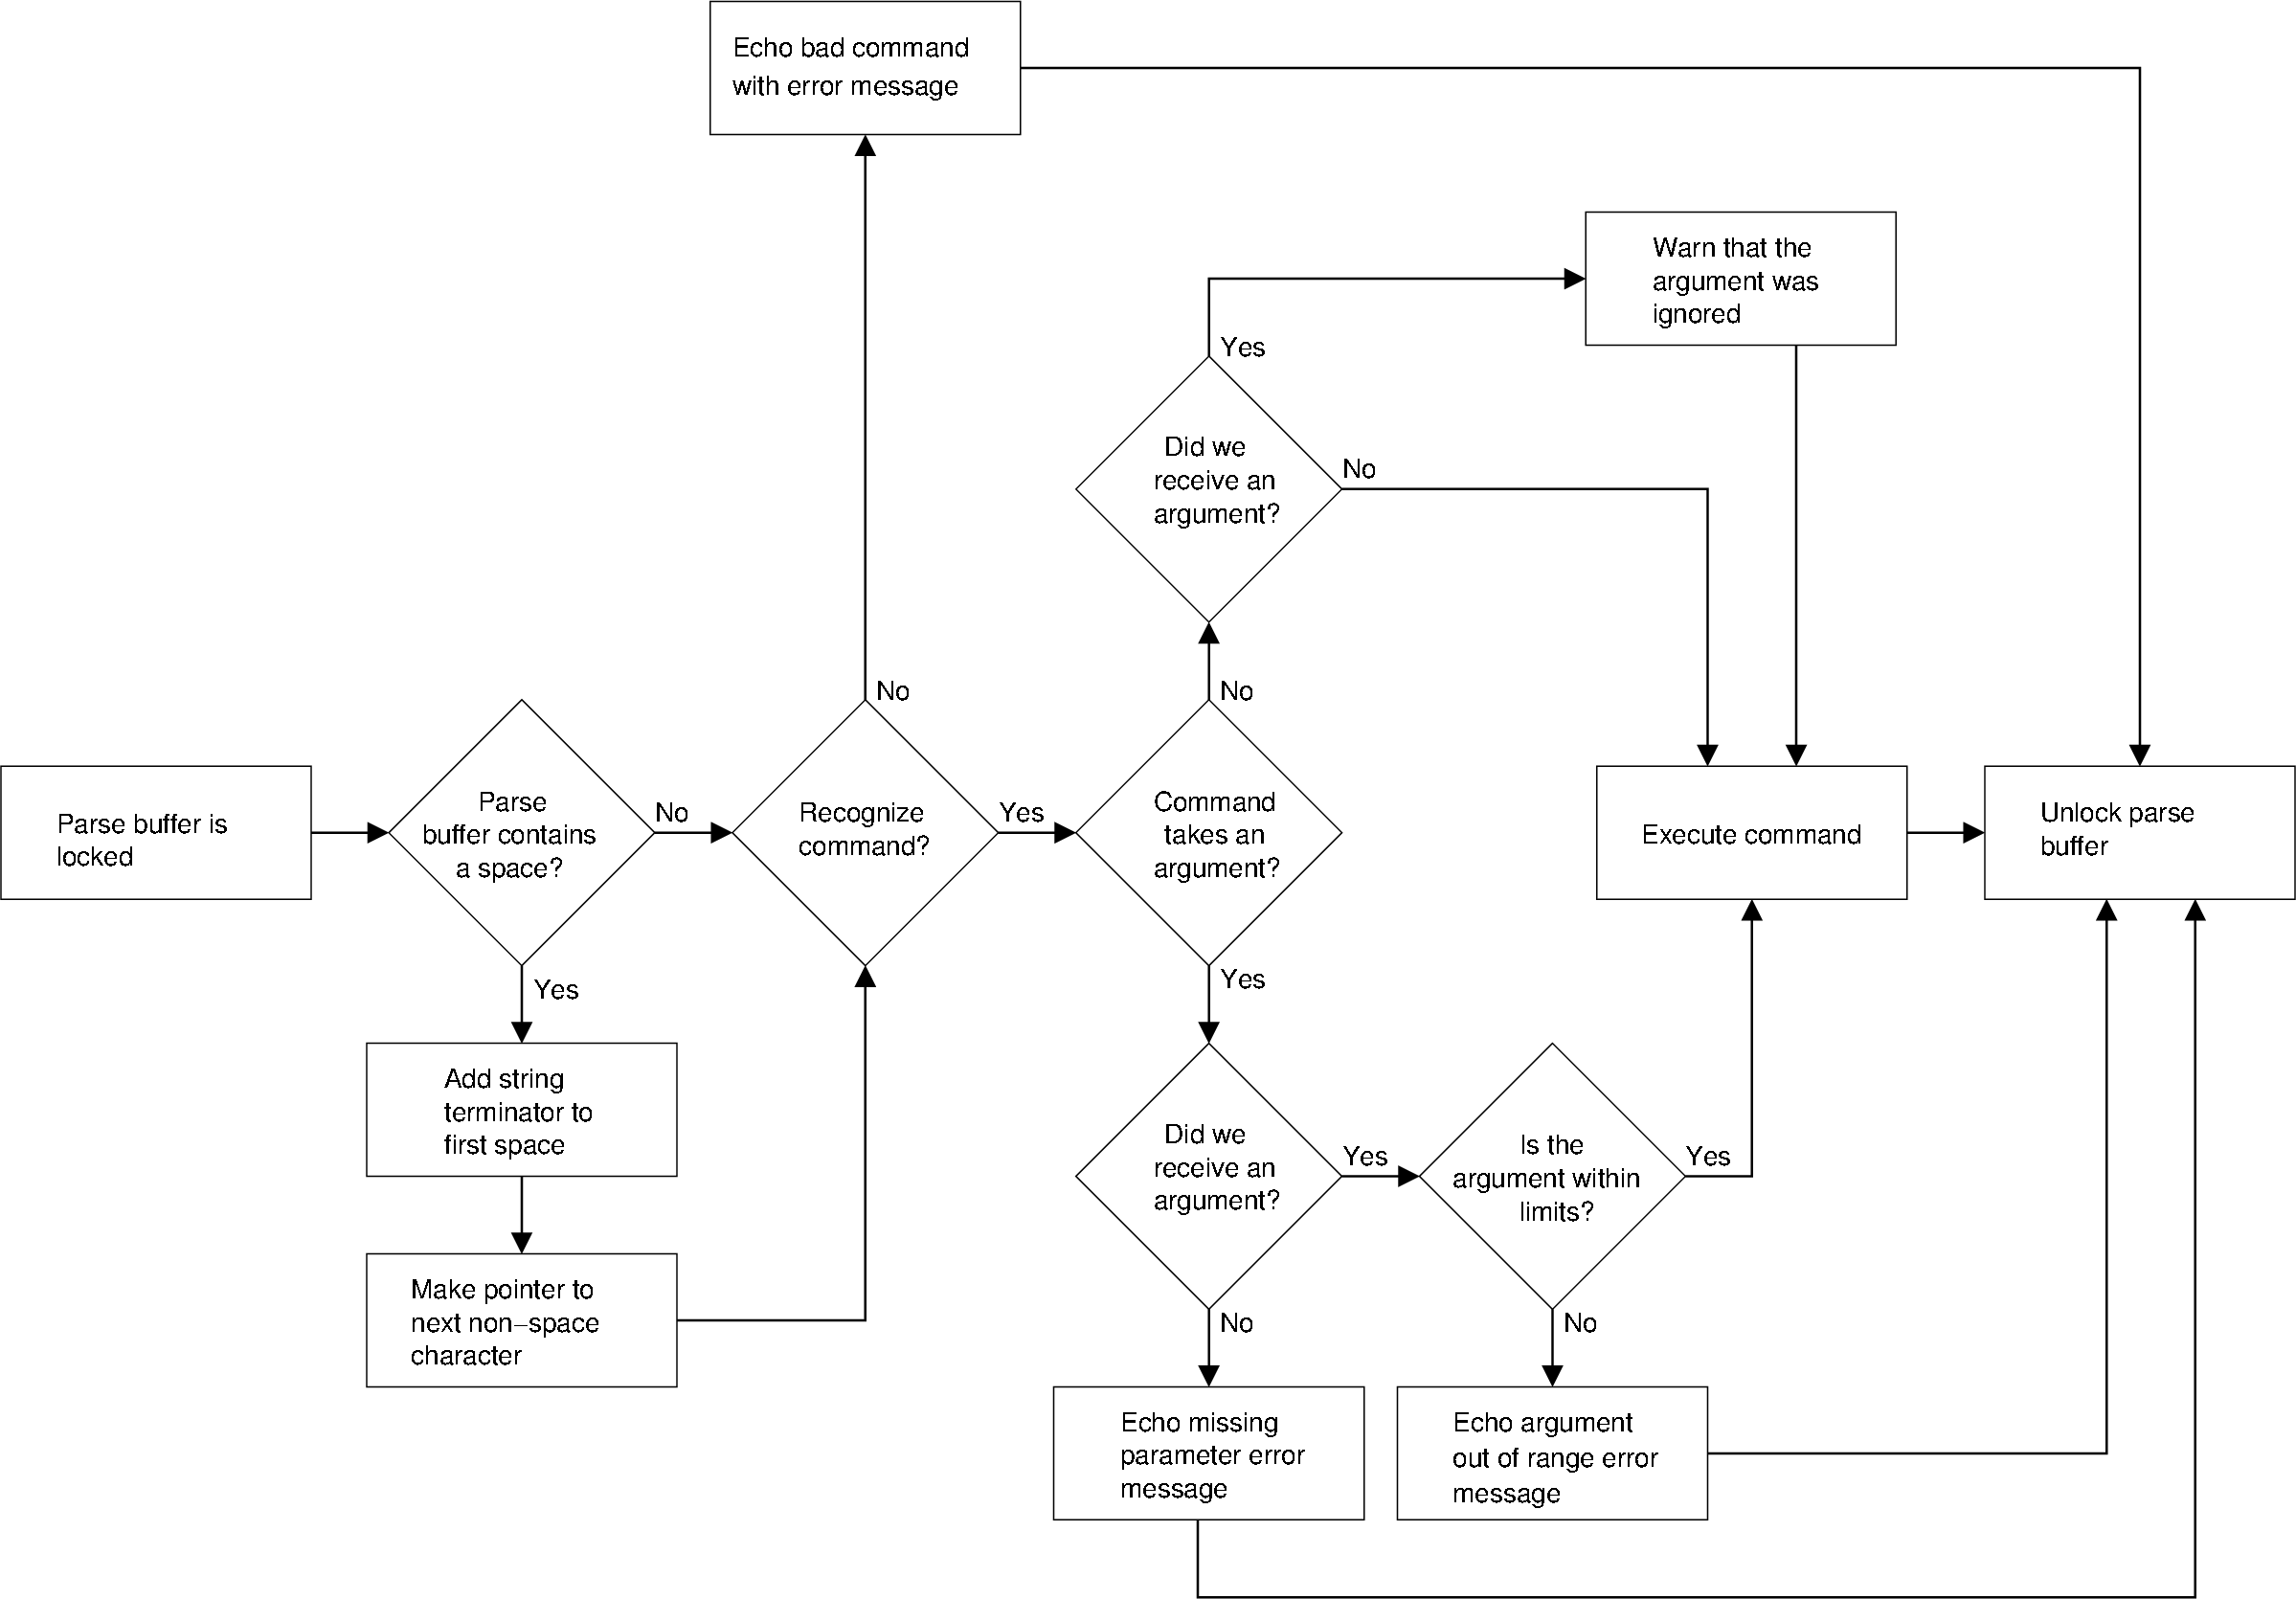
\includegraphics[clip,scale=0.7]{./tikz/parse_cmd_flow}
        \draftnote{parse\_cmd\_flow.tex}
        \caption{Program flow for processing fully-formed commands.  This processing step happens in the main loop, so it will only run when the system isn't busy doing something else.  Notice that all incoming commands are converted to lowercase, so there's no case sensitivity.\label{fig:cmdflow}}
    \end{center}
\end{figure}

% The parse buffer figure showing command and argument strings
\begin{figure}[ht]
    \begin{center}
        \includegraphics[clip,scale=1]{prsbuffer}
        \draftnote{prsbuffer.fig}
        \caption{The parse buffer with pointers to the command and argument strings.  The single combined string copied from the receive buffer is made into two strings by inserting a string terminator.\label{fig:prsbuffer}}
    \end{center}
\end{figure}

% The command snippet figure is created with two text files (command_array.txt
% and command_type.txt) individually converted to fig format using code2fig.sh
% and then combined into one fig file.
\begin{listing}[ht]
    \begin{center}
        \includegraphics[clip,scale=0.75]{command_snippet}
        \draftnote{command\_snippet.fig}
        \caption{Code snippets from two files show how the command structure is defined (upper), and how commands are initialized (lower).  When the command processor is run, commands in the parse buffer are matched with names from the command array.  Commands can be added to the system by adding to this array of command types.\label{lst:cmdsnip}}
    \end{center}
\end{listing}

\clearpage{}
\section{Adding more commands}
Since being able to extend this system is so important, I've come up with a procedure for adding new commands.  First, choose the name of your command.  This can be harder than it sounds.  I like names to be short enough to be easily entered on the command line, but long enough to be descriptive.  The name can contain any ASCII character except a space.  Remember that the command characters, the argument characters, one space, and one string terminator must all fit in the received character buffer.
    
Next, decide whether or not you need more than a hexadecimal integer string argument.  My argument handling ability is limited to just hexadecimal integer strings.  Extending the system isn't hard, but remember that every function called by a command has to accept the same arguments.  If you add a character pointer argument, even commands that take no arguments must then call functions that need both integer and character pointer arguments.  This can be tedious if you already have a lot of commands defined.

If your arguments fit your ability to handle them, add a function for your command to call.  You might like to put all the functions called by remote commands in their own module.  I don't worry too much about this, but I do try to prefix names with ``cmd\_'' if those functions are called exclusively by remote commands.  This helps me remember that their arguments and return value are fixed.

Now that the command's attributes have been specified, it's time to give it an entry in the command array.  Add the new entry before the array's end marker.  You've already chosen the command's name, argument type, and function call.  The remaining entry members are the argument's maximum size in characters and the command's help string.  Remember that hexadecimal arguments larger than 4 characters don't make sense for 16-bit integers.  As for the help strings, I was only able to use the PROGMEM macro on them if I defined them outside of the command array.  This breaks up the array organization, but these strings will quickly eat up the Butterfly's RAM if they're not located and referenced in flash.  


\clearpage{}
\section{Conclusion: Is there any space left?}
I built the code with avr-gcc, using the -Os optimization level.  The output of \textbf{avr-gcc --version} is: \texttt{avr-gcc (Gentoo 4.6.3 p1.3, pie-0.5.1) 4.6.3}. The resulting memory map file shows a \texttt{.data} size of 182 bytes, a \texttt{.bss} size of 100 bytes, and a \texttt{.text} size of 7.5 kilobytes.  I'm using roughly half of the Butterfly's flash and a third of its RAM.  So there's at least some space left to do something else with the Butterfly besides using it to recognize commands.  I'm most excited for the time when I don't have to think about this C code anymore, and can focus on using the Butterfly as a peripheral for the PC.  Until then, I hope somebody can learn from my experience.

\section{Biography}
John Peck is a design engineer at Stanford Research Systems in Sunnyvale, CA.  He has been using ASCII interfaces to test equipment since he was a graduate student at the University of Wisconsin at Madison.  He can be reached at \texttt{john@johnpeck.info}.


\clearpage{}
\raggedright
\bibliography{doctools/latex/hydrorefs}
\end{document}
